\documentclass[border=5pt]{standalone}
\usepackage[utf8x]{inputenc}
\usepackage[english]{babel}

% enables flowchart drawing
\usepackage{tikz}
\usetikzlibrary{shapes.geometric, arrows}

\tikzstyle{startstop} = [rectangle, rounded corners, minimum width=3cm, minimum height=1cm,text centered, text width = 3.5cm, draw=black, fill=gray!60]
\tikzstyle{process} = [rectangle, minimum width = 3cm, minimum height = 1.5cm, text centered, text width = 3.5cm, draw=black, fill = gray!10]
\tikzstyle{decision} = [diamond, minimum width = 3cm, minimum height = 2cm, text centered, text width = 3cm, draw=black, fill = gray!35, inner sep=-0.2ex, aspect = 1.5]
\tikzstyle{arrow} = [thick,->,>=stealth]



\begin{document}

\begin{footnotesize}
	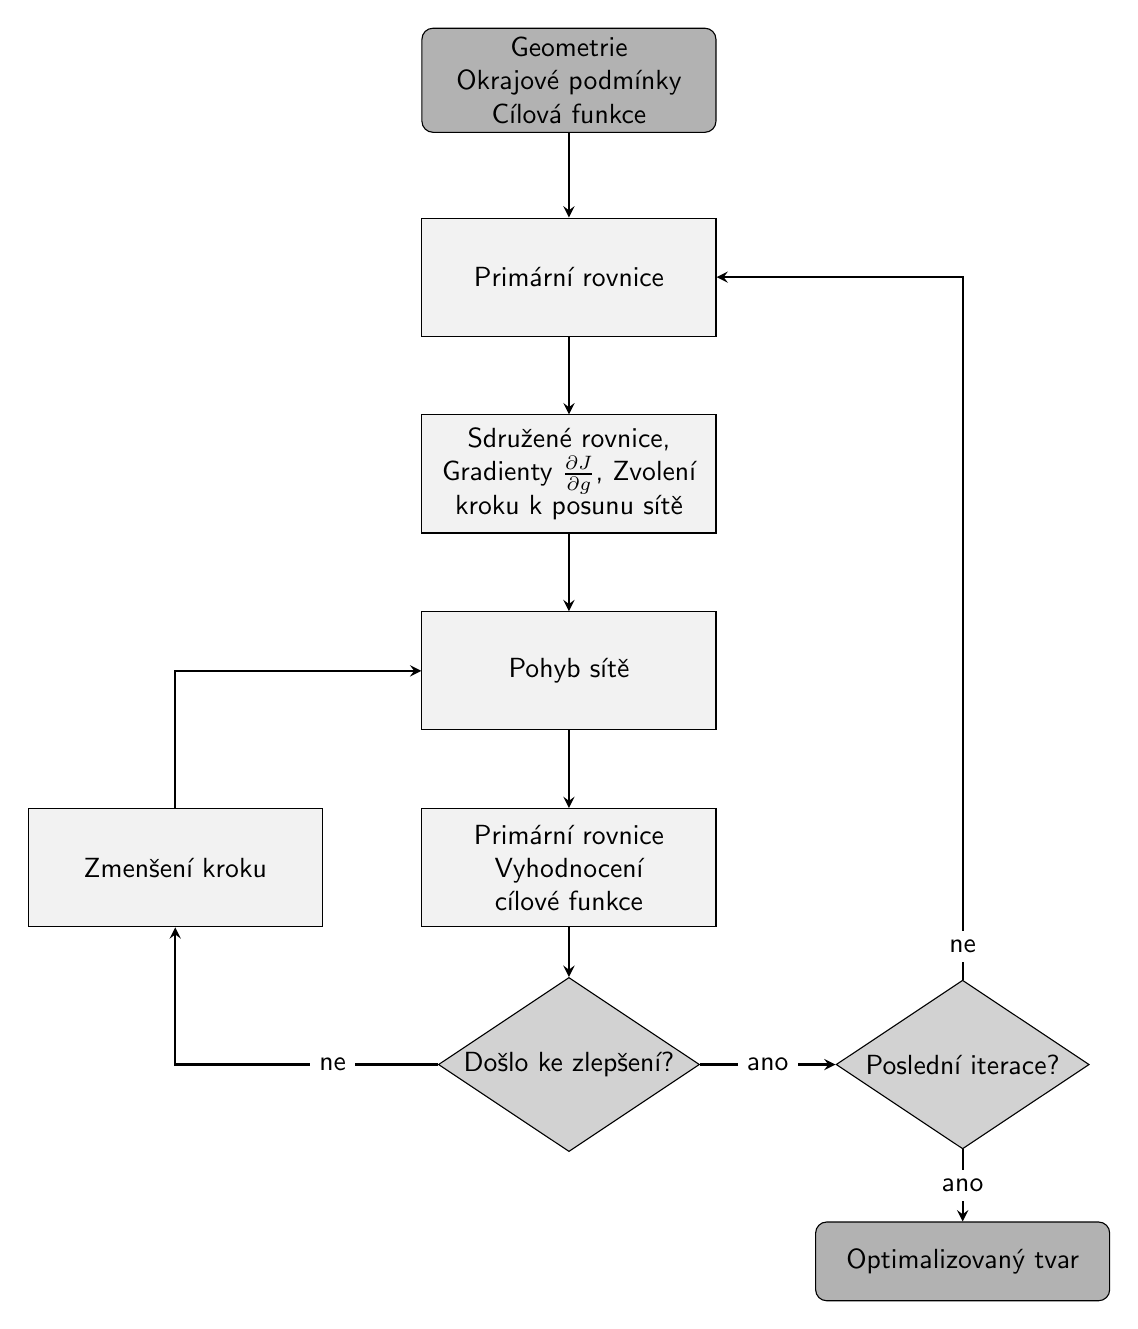
\begin{tikzpicture}[node distance=2cm, every node/.style={fill=white, font=\sffamily}]
	\node (B1) [startstop] {Geometrie
		
		 Okrajové podmínky
		 
		 Cílová funkce};
	
	\node (B2) [process, below of = B1, yshift = -0.5cm] {Primární rovnice};
	\node (B3) [process, below of = B2, yshift = -0.5cm] {Sdružené rovnice, Gradienty $ \frac{\partial J}{\partial g} $, Zvolení kroku k posunu sítě };
%	\node (B4) [process, below of = B3, yshift = -0.5cm] { };
%	\node (B5) [process, below of = B4, yshift = -0.5cm] { };
	\node (B6) [process, below of = B3, yshift = -0.5cm] { Pohyb sítě };
	\node (B7) [process, below of = B6, yshift = -0.5cm] { Primární rovnice
		
		 Vyhodnocení cílové funkce };
%	\node (B8) [process, below of = B7, yshift = -0.5cm] {  };
	\node (B9) [decision, below of = B7, yshift = -0.5cm] { Došlo ke zlepšení? };
	\node (B10) [process, left of = B7, xshift = -3cm] { Zmenšení kroku };
	\node (B11) [decision, right of = B9, xshift = 3cm] { Poslední iterace?};
	\node (B12) [startstop, below of = B11, yshift = -0.5cm] {Optimalizovaný tvar};
	
	
%	\node (B3) [process, right of = B2, xshift = 3cm] {Velocity triangles at the impeller inlet};
%	\node (B4) [process, below of = B3, yshift = -0.5cm] {Incidence loss};
%	\node (B5) [process, left of = B4, xshift = -3cm] {Head enthalpy and outlet density estimation};
%	\node (B6) [process, left of = B5, xshift = -4cm] {Internal losses};
%	\node (B7) [process, below of = B6, yshift = -0.5cm] {Outlet density calculation};
%	\node (B8) [decision, below of = B7, yshift = -0.5cm] { $\rho_{2, est} = \rho_{2, calc}$ ?};
%	\node (B9) [process, right of = B8, xshift = 4cm] {External losses};
%	\node (B10) [process, right of = B9, xshift = 3cm] {Vaneless diffuser loss};
%	\node (B11) [startstop, above of = B10, yshift = 0.5cm] {Performance parameters};
	
				\draw [arrow] (B1)--(B2);
				\draw [arrow] (B2)--(B3);
				\draw [arrow] (B3)--(B6);
%				\draw [arrow] (B4)--(B5);
%				\draw [arrow] (B5)--(B6);
				\draw [arrow] (B6)--(B7);
				\draw [arrow] (B7)--(B9);
%				\draw [arrow] (B8)--(B9);
				\draw [arrow] (B9)-- ++(-3,0) node {ne}-|(B10);
				\draw [arrow] (B10) |-(B6);
				\draw [arrow] (B9)-- node {ano} (B11);
				\draw [arrow] (B11)-- ++(0,1.5) node {ne} |-   (B2);
				\draw [arrow] (B11) -- node {ano} (B12);
				
%				\draw [arrow] (B9) -- ++(3,0) -- ++(0,12.5) -- ++(-1.15,0)  (B2);
				
%				\draw [arrow] (B10)--(B11);
%				\draw [arrow] (3, -7.5)--(3, -2.5);
	
%				\node[right] at (3, -5) {no};
%				\node[below] at (3, -7.5) {yes};
	\end{tikzpicture}
\end{footnotesize}

\end{document}